\section{Risultati}
\label{sec:results}

Tutti i valori numerici provengono dagli array \code{.npz} salvati dai runner e sono
calcolati da \code{make\_report\_tables.py}.

% =====================================================================
\subsection{CartPole --- controllo: Q-Learning vs SARSA}
\label{sec:res-cartpole-control}

Entrambi gli algoritmi apprendono in modo netto (Fig.~\ref{fig:cp-control},
Tab.~\ref{tab:cartpole-control}): da $\approx 27$--$41$ arrivano a \res{223.6}{49.4}
(Q\hbox{-}Learning) e \res{258.3}{31.1} (SARSA). Due osservazioni contano pi\`u dei
numeri assoluti.

\textbf{Le curve sono ancora in salita a fine budget}: a 10\,000 episodi nessuna ha
raggiunto un plateau, e il massimo dell'ambiente \`e 500. Il vincolo \`e il budget, non
l'algoritmo: la griglia a $10^4$ stati va esplorata quasi tutta.

\textbf{SARSA supera Q\hbox{-}Learning ed \`e meno disperso tra seed} ($\pm 31$ contro
$\pm 49$) --- l'opposto dell'intuizione, dato che Q\hbox{-}Learning apprende la policy
\emph{ottima}. La spiegazione: la curva misura la performance \emph{durante} il
training, con $\varepsilon = 0.1$ attivo. Q\hbox{-}Learning valuta la policy greedy e
ignora che il $10\%$ delle volte far\`a una mossa casuale; SARSA include quel rischio
nel target e impara una policy che tollera le proprie deviazioni. Dove una singola
azione sbagliata fa cadere l'asta, tenerne conto paga: \`e la dinamica del CliffWalking
(S\&B Fig.~6.5), attenuata ma visibile.

\begin{figure}[htbp]
\centering
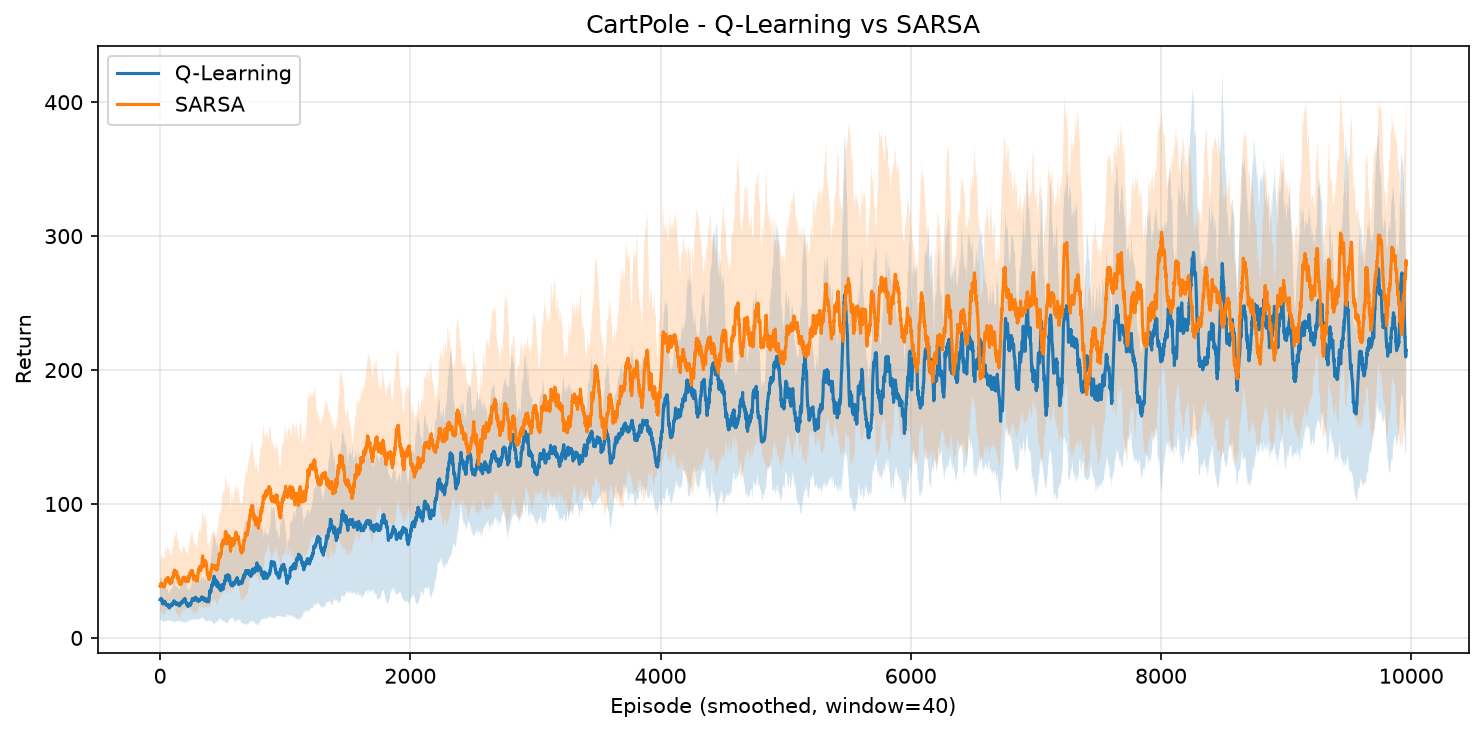
\includegraphics[width=0.55\linewidth]{cartpole_control_comparison.png}
\caption{CartPole: Q\hbox{-}Learning vs SARSA a parit\`a di iperparametri (media su 3
seed, banda $\pm1\sigma$). SARSA (arancio) sta sopra per tutto il training; entrambe le
curve salgono ancora a 10\,000 episodi.}
\label{fig:cp-control}
\end{figure}

\begin{table}[htbp]
\centering
\caption{CartPole, controllo: Q-Learning vs SARSA a parit\`a di iperparametri ($\alpha=0.1$, $\gamma=0.99$, $\varepsilon=0.1$), media su 3 seed. Il return massimo dell'ambiente \`e 500; entrambe le curve sono ancora in salita a fine budget.}
\label{tab:cartpole-control}
\begin{tabular}{lccc}
\toprule
Algoritmo & Return iniziale & Return finale & Episodi/seed \\
          & (primi 100 ep) & (ultimo 10\% ep, media $\pm$ std) & \\
\midrule
Q-Learning & 26.6 & $223.6 \pm 49.4$ & 10000 \\
SARSA & 40.8 & $258.3 \pm 31.1$ & 10000 \\
\bottomrule
\end{tabular}
\end{table}


% =====================================================================
\subsection{CartPole --- sensibilit\`a a $\varepsilon$, $\alpha$, $\gamma$}
\label{sec:res-cartpole-sens}

La Fig.~\ref{fig:cp-sens} riporta le sei sweep. Averle
fatte per \emph{entrambi} gli algoritmi non \`e ridondanza: su $\alpha$ i due si
comportano diversamente, ed \`e il dato pi\`u interessante della sezione.

\begin{itemize}
  \item \textbf{$\gamma$ --- l'effetto pi\`u netto.} Valori alti vincono per entrambi:
        $\gamma \in \{0.99, 1.0\}$ arriva a $230$--$280$, $\gamma \in \{0.9, 0.95\}$ si
        blocca a $140$--$165$. Strutturale: CartPole \`e un compito di
        \emph{sopravvivenza} con reward $+1$/passo, quindi il valore di uno stato
        \emph{\`e} quanto a lungo si sopravvive. Con $\gamma=0.9$ l'orizzonte effettivo
        \`e $\approx 1/(1-\gamma) = 10$ passi: l'agente non pu\`o vedere la caduta che
        sta preparando.
  \item \textbf{$\varepsilon$ --- serve, ma il troppo non nuoce.} $\varepsilon=0.01$ \`e
        il peggiore per entrambi ($105$--$130$), mentre $\varepsilon=0.3$ \emph{non}
        degrada ($220$--$250$, come $0.1$): il reward denso perdona l'esplorazione,
        perch\'e una mossa casuale costa al pi\`u qualche passo. Su Acrobot accadr\`a
        l'esatto contrario (Sez.~\ref{sec:res-acrobot-eps}): l'effetto di $\varepsilon$
        dipende dalla struttura del reward, non \`e una propriet\`a dell'algoritmo.
  \item \textbf{$\alpha$ --- qui i due divergono.} Per Q\hbox{-}Learning $\alpha=0.5$ e
        $\alpha=0.1$ finiscono appaiati ($200$--$220$), con $0.5$ pi\`u veloce
        all'inizio. Per \emph{SARSA} invece $\alpha=0.5$ parte forte ma
        \textbf{satura sotto} $\alpha=0.1$ ($\approx 210$ contro $\approx 260$). SARSA
        \`e on-policy, quindi il target $Q(S',A')$ contiene la casualit\`a dell'azione
        $A'$: un $\alpha$ alto insegue quel rumore invece di mediarlo.
        Q\hbox{-}Learning, che usa il $\max$ (deterministico dato $Q$), ne soffre meno.
        $\alpha=0.01$ \`e troppo lento per entrambi ($45$--$95$).
\end{itemize}

\begin{figure}[htbp]
\centering
\begin{subfigure}{0.31\linewidth}
  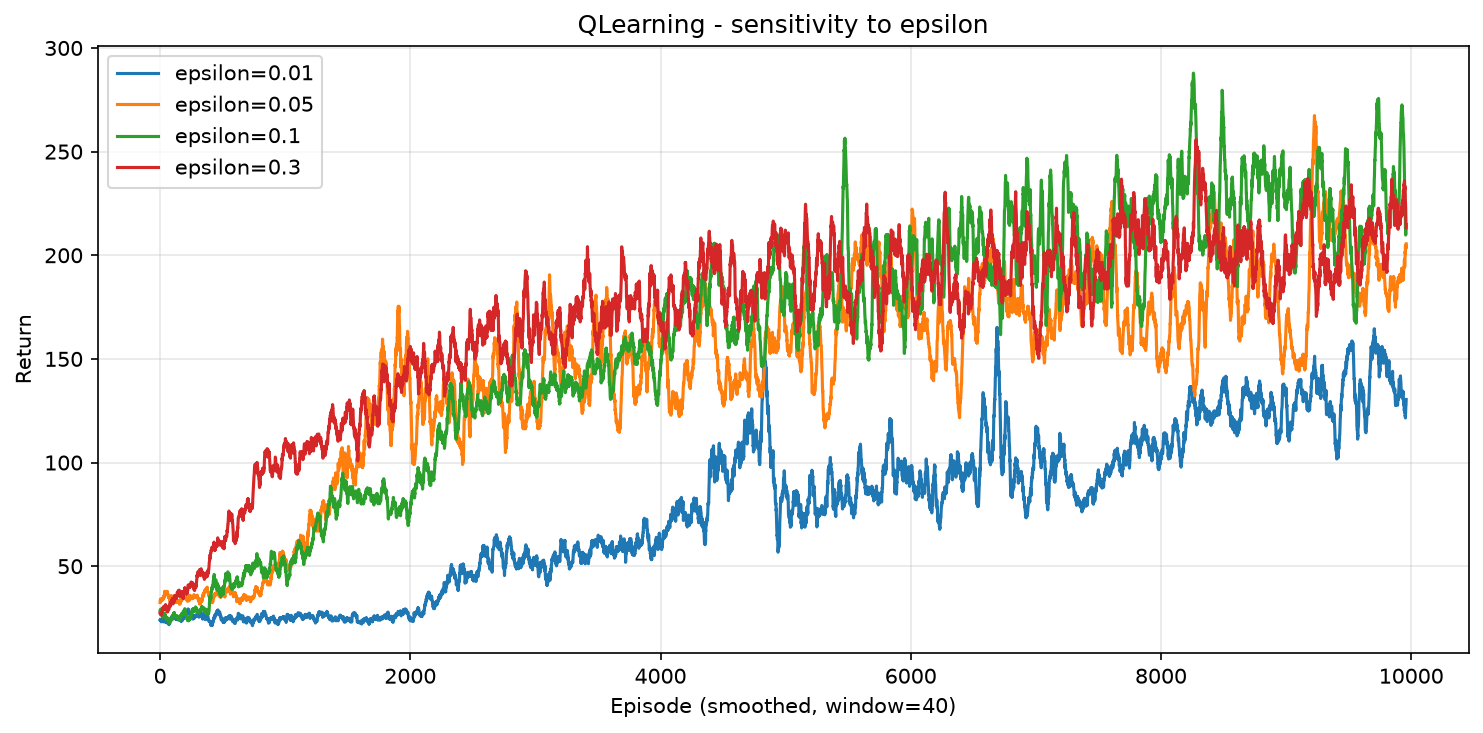
\includegraphics[width=\linewidth]{cartpole_sensitivity_QLearning_epsilon.png}
  \caption{Q-Learning, $\varepsilon$}
\end{subfigure}\hfill
\begin{subfigure}{0.31\linewidth}
  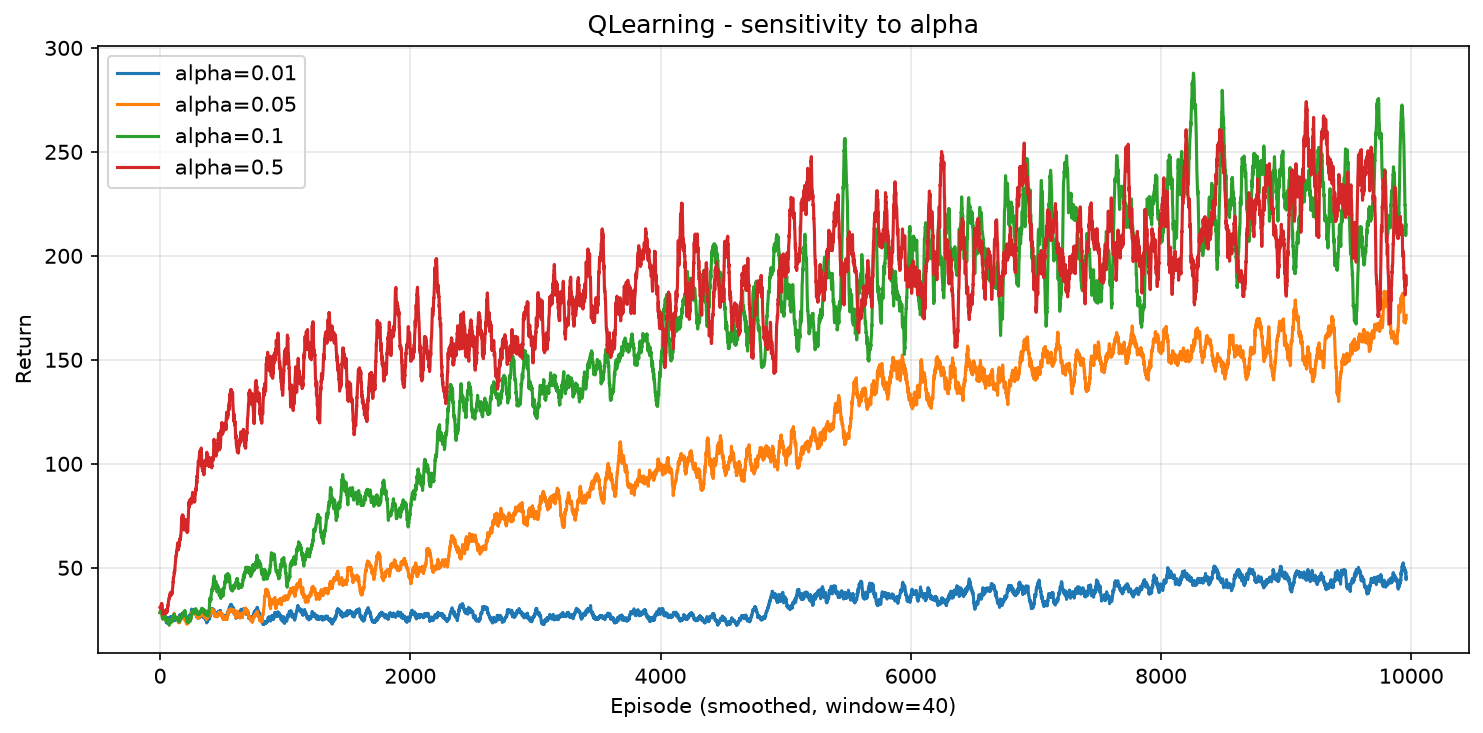
\includegraphics[width=\linewidth]{cartpole_sensitivity_QLearning_alpha.png}
  \caption{Q-Learning, $\alpha$}
\end{subfigure}\hfill
\begin{subfigure}{0.31\linewidth}
  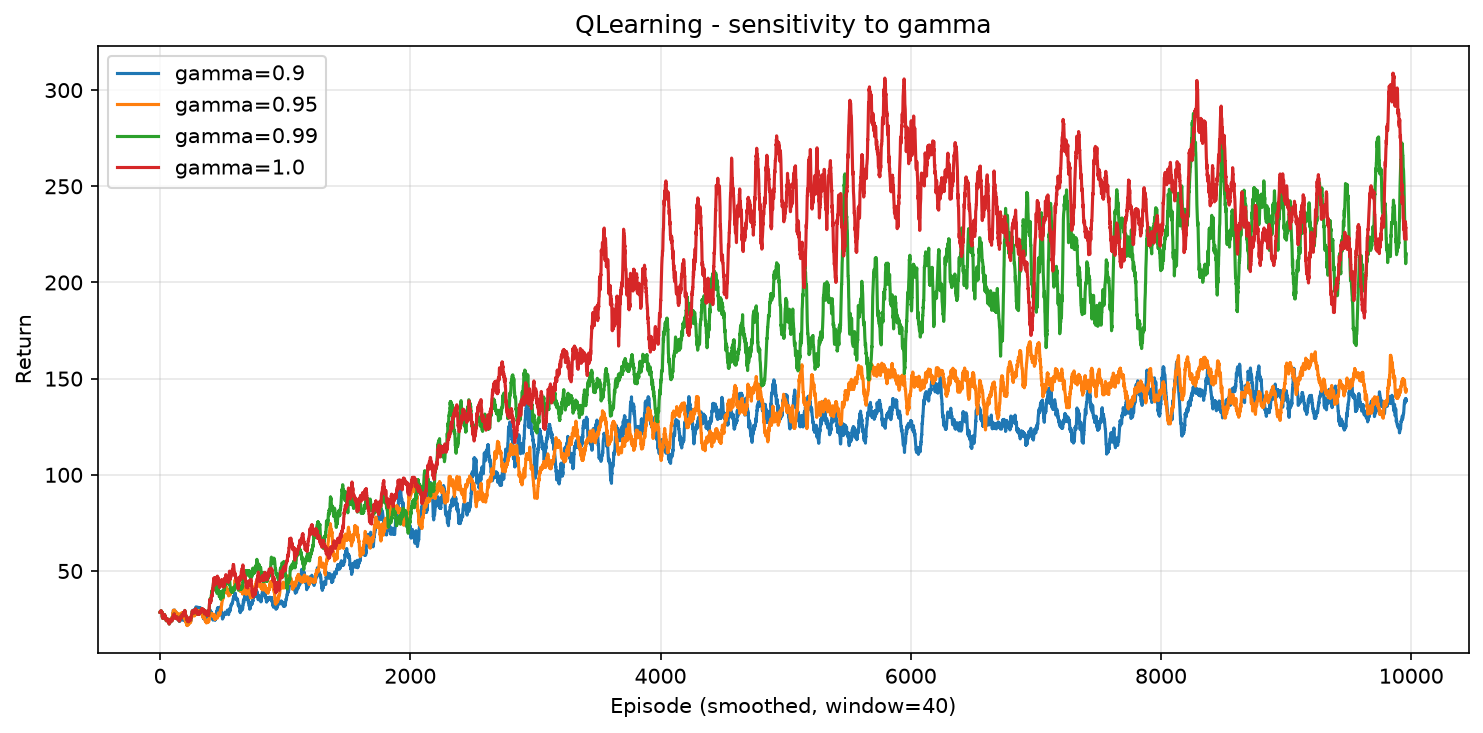
\includegraphics[width=\linewidth]{cartpole_sensitivity_QLearning_gamma.png}
  \caption{Q-Learning, $\gamma$}
\end{subfigure}

\medskip
\begin{subfigure}{0.31\linewidth}
  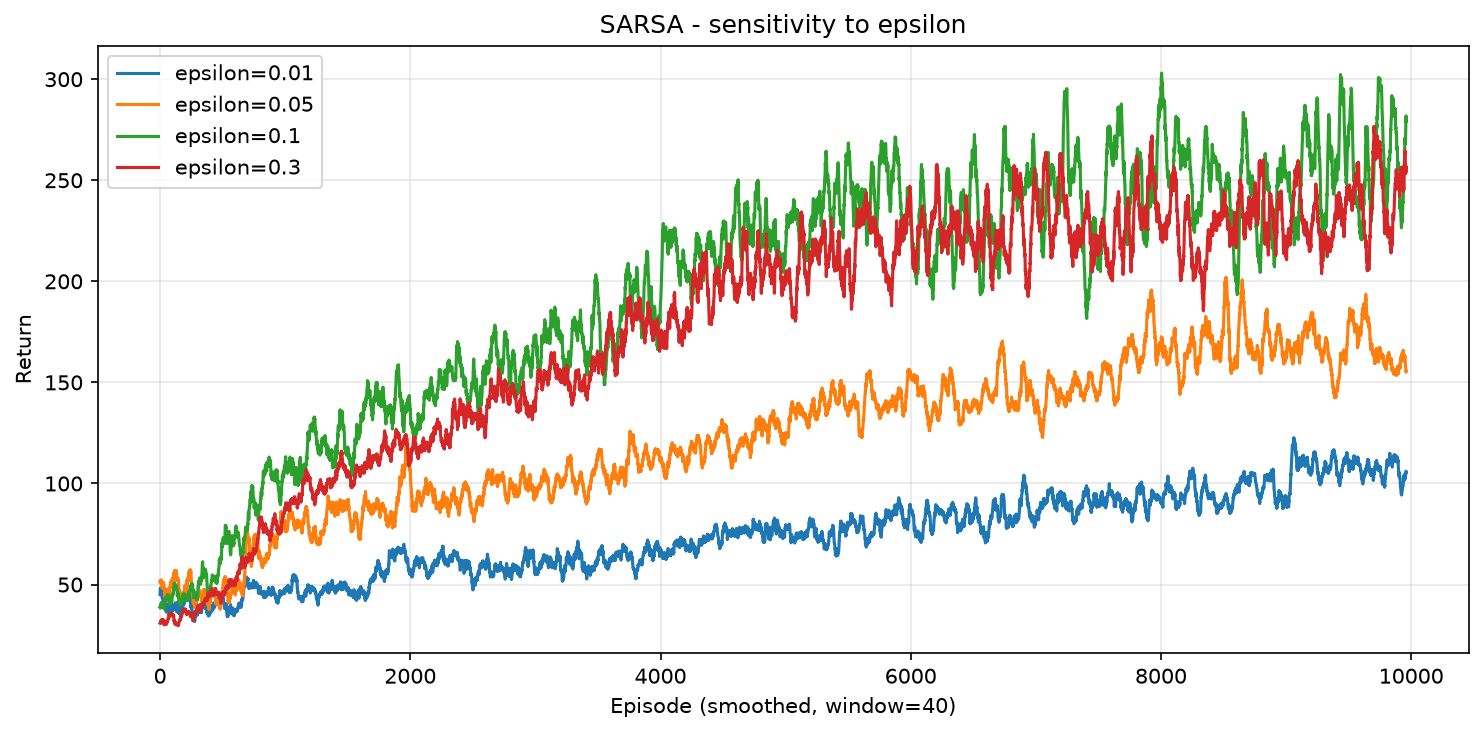
\includegraphics[width=\linewidth]{cartpole_sensitivity_SARSA_epsilon.png}
  \caption{SARSA, $\varepsilon$}
\end{subfigure}\hfill
\begin{subfigure}{0.31\linewidth}
  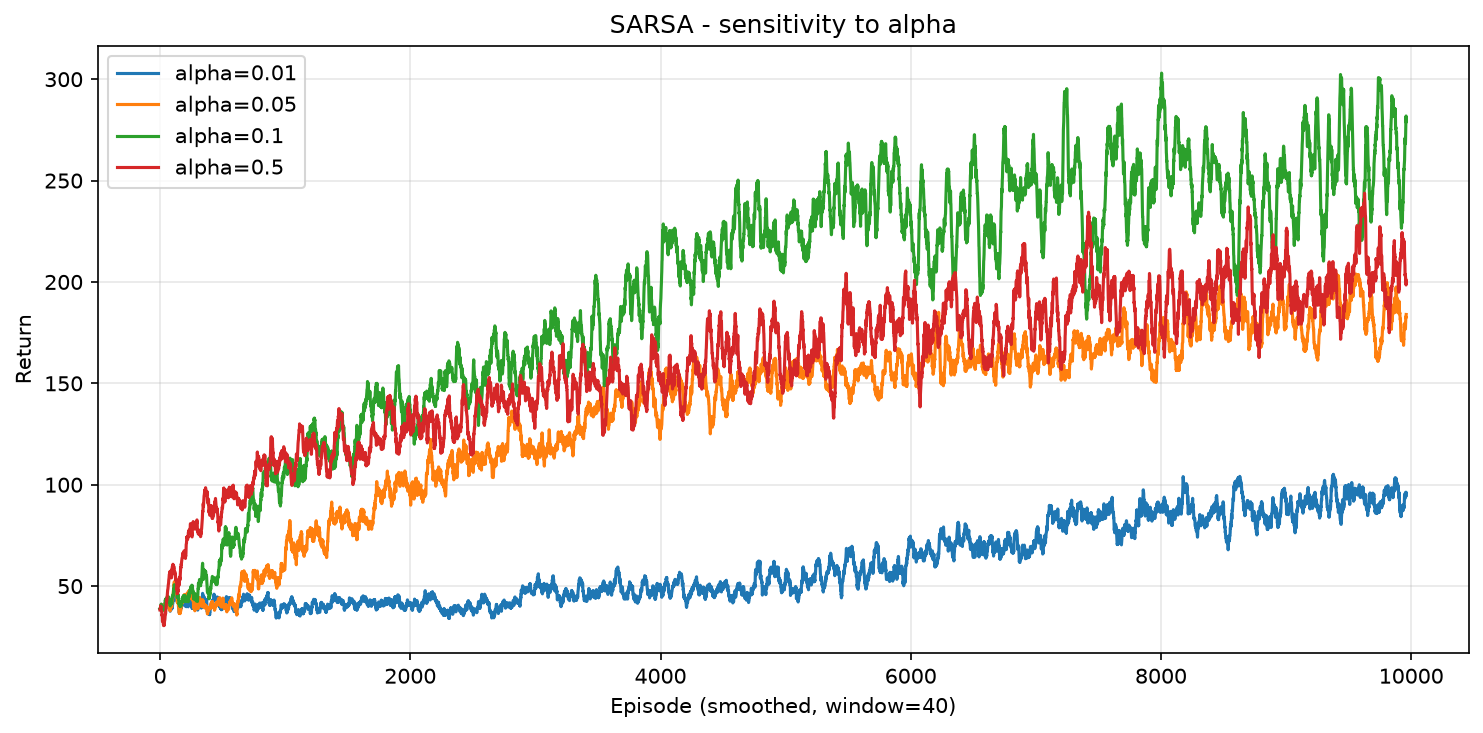
\includegraphics[width=\linewidth]{cartpole_sensitivity_SARSA_alpha.png}
  \caption{SARSA, $\alpha$}
\end{subfigure}\hfill
\begin{subfigure}{0.31\linewidth}
  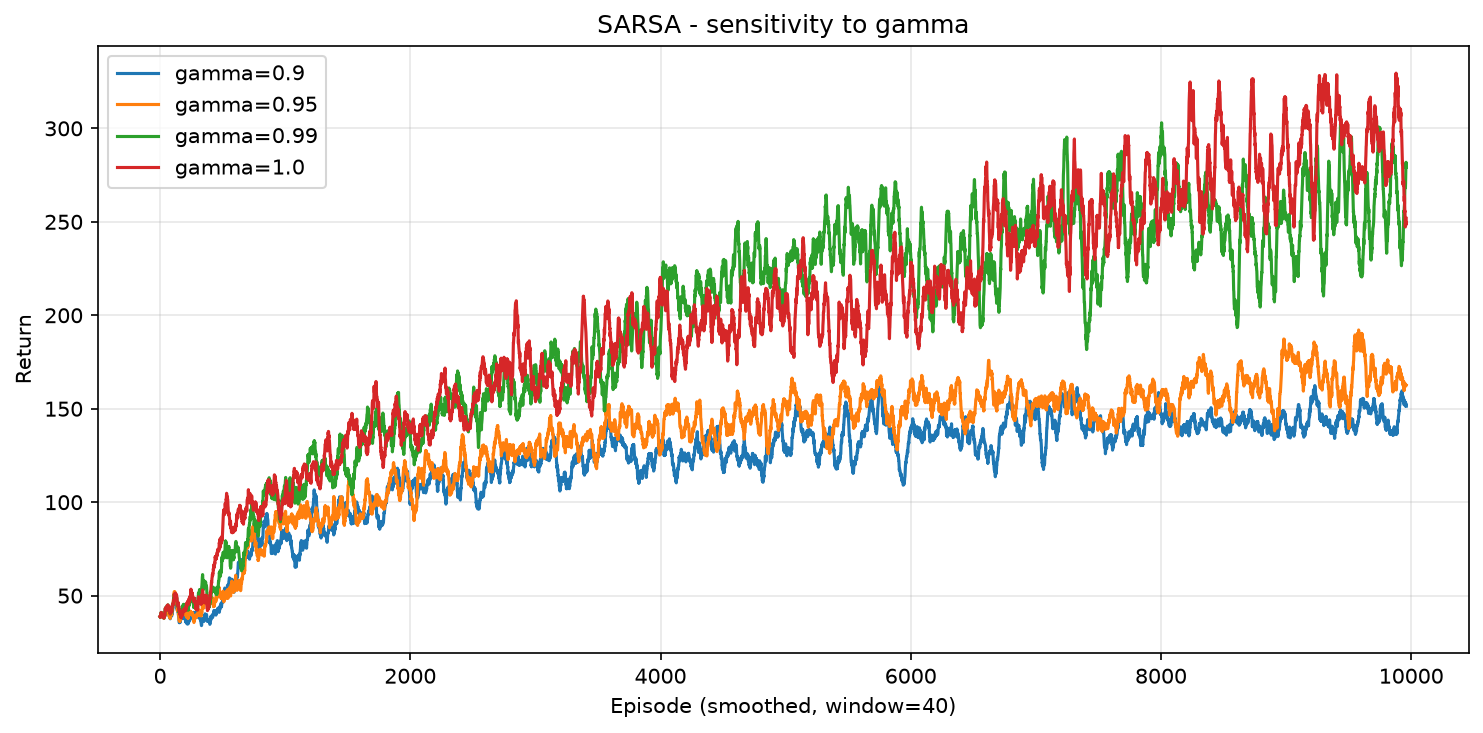
\includegraphics[width=\linewidth]{cartpole_sensitivity_SARSA_gamma.png}
  \caption{SARSA, $\gamma$}
\end{subfigure}
\caption{CartPole: le sei sweep di sensibilit\`a (media su 3 seed; bande omesse per
leggibilit\`a, Sez.~\ref{sec:experiments-reading}). Riga superiore Q\hbox{-}Learning,
inferiore SARSA. $\gamma$ alto domina in entrambi; $\varepsilon$ troppo basso \`e il vero
problema, mentre $\varepsilon=0.3$ non danneggia. La differenza tra i due algoritmi sta
nel pannello $\alpha$: per SARSA (e) $\alpha=0.5$ (rosso) parte veloce ma satura
\emph{sotto} $\alpha=0.1$ (verde), mentre per Q\hbox{-}Learning (b) i due si equivalgono.}
\label{fig:cp-sens}
\end{figure}

% =====================================================================
\subsection{CartPole --- $\varepsilon$ costante vs annealing}
\label{sec:res-cartpole-anneal}

Mi aspettavo che l'annealing servisse a poco su CartPole, che ha reward denso e non \`e
limitato dall'esplorazione. Il beneficio c'\`e, ma \`e soprattutto sulla
\emph{stabilit\`a}: l'annealing ($1.0 \to 0.01$) chiude a \res{243.8}{23.9} contro
\res{223.6}{49.4} del costante (Fig.~\ref{fig:cp-anneal}). Il guadagno in media \`e
modesto ($+20$), ma la dispersione tra seed si \emph{dimezza}: ridurre $\varepsilon$ a
fine training toglie il rumore che la policy si porta dietro, e l'esito dipende meno dal
seed. Il prezzo \`e un avvio pi\`u lento, fino a $\approx 3500$ episodi.

\begin{figure}[htbp]
\centering
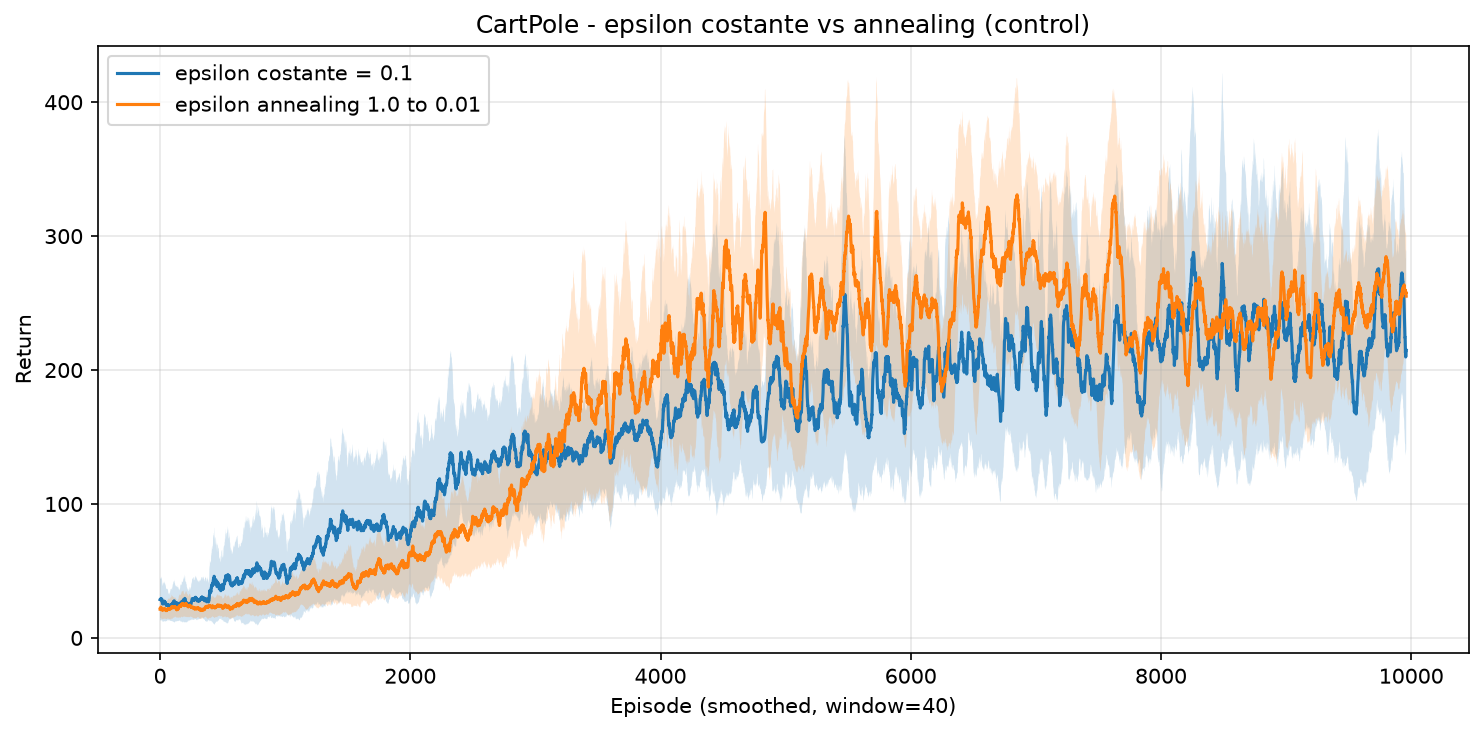
\includegraphics[width=0.55\linewidth]{cartpole_epsilon_annealing.png}
\caption{CartPole: $\varepsilon$ costante $=0.1$ vs annealing $1.0 \to 0.01$.
L'annealing paga un avvio pi\`u lento, poi sorpassa e chiude con banda $\pm1\sigma$
visibilmente pi\`u stretta.}
\label{fig:cp-anneal}
\end{figure}

% =====================================================================
\subsection{CartPole --- MC vs TD(0): bias, varianza, stabilit\`a}
\label{sec:res-cartpole-pred}

\textbf{Il return non pu\`o distinguere i due stimatori} (Fig.~\ref{fig:cp-pred}a): le
curve sono \emph{identiche per costruzione}, perch\'e MC e TD(0) valutano la
\emph{stessa} policy fissa e generano quindi gli stessi episodi (return $\approx 330$).
La curva di MC \`e letteralmente nascosta sotto quella di TD. Non \`e un errore di
plotting: \`e la prova che la differenza tra i due metodi non vive nel return ma nelle
stime $V(s)$. Per inciso, quei $\approx 330$ passi sono ottenuti dalla policy greedy
\emph{senza} esplorazione, contro i $\approx 224$ della curva di training: gran parte
del divario dal massimo \`e il costo di $\varepsilon$, non incapacit\`a della policy.

\textbf{La differenza vive nelle stime} (Fig.~\ref{fig:cp-pred}b), ed \`e il quadro
classico di S\&B \S6.2. \textbf{MC} salta al valore corretto ($81.07 \pm 0.17$) in poche
decine di episodi ma con un picco iniziale violento: \`e \emph{non distorto} e ad
\emph{alta varianza}, perch\'e ogni aggiornamento usa il return completo di una
traiettoria di $\approx 330$ passi. \textbf{TD(0)} parte da 0 e sale lentamente e in modo
liscio, fermandosi a $70.50 \pm 0.28$ dopo 6000 episodi --- ancora $13\%$ sotto MC: \`e
\emph{distorto} (fa bootstrap su una stima ancora sbagliata) ma a \emph{bassa varianza}.

\textbf{Il bias di TD(0) non \`e una costante: dipende dalla policy valutata.} \`E il
risultato che giustifica l'aver valutato anche la policy casuale
(Fig.~\ref{fig:cp-pred-random}). L\`i gli episodi durano $\approx 22$ passi, lo stato di
riferimento \`e vicinissimo alla terminazione, e TD(0) \emph{raggiunge} MC entro
$\approx 5000$ episodi ($17.04$ contro $17.43$): il bias sparisce. Con la policy appresa
gli episodi sono quindici volte pi\`u lunghi e il bootstrap deve propagare il valore un
passo alla volta. La distorsione di TD(0) \`e quindi una funzione della \emph{distanza
temporale} tra lo stato e il reward, non un difetto fisso dell'algoritmo.

\begin{figure}[htbp]
\centering
\begin{subfigure}{0.46\linewidth}
  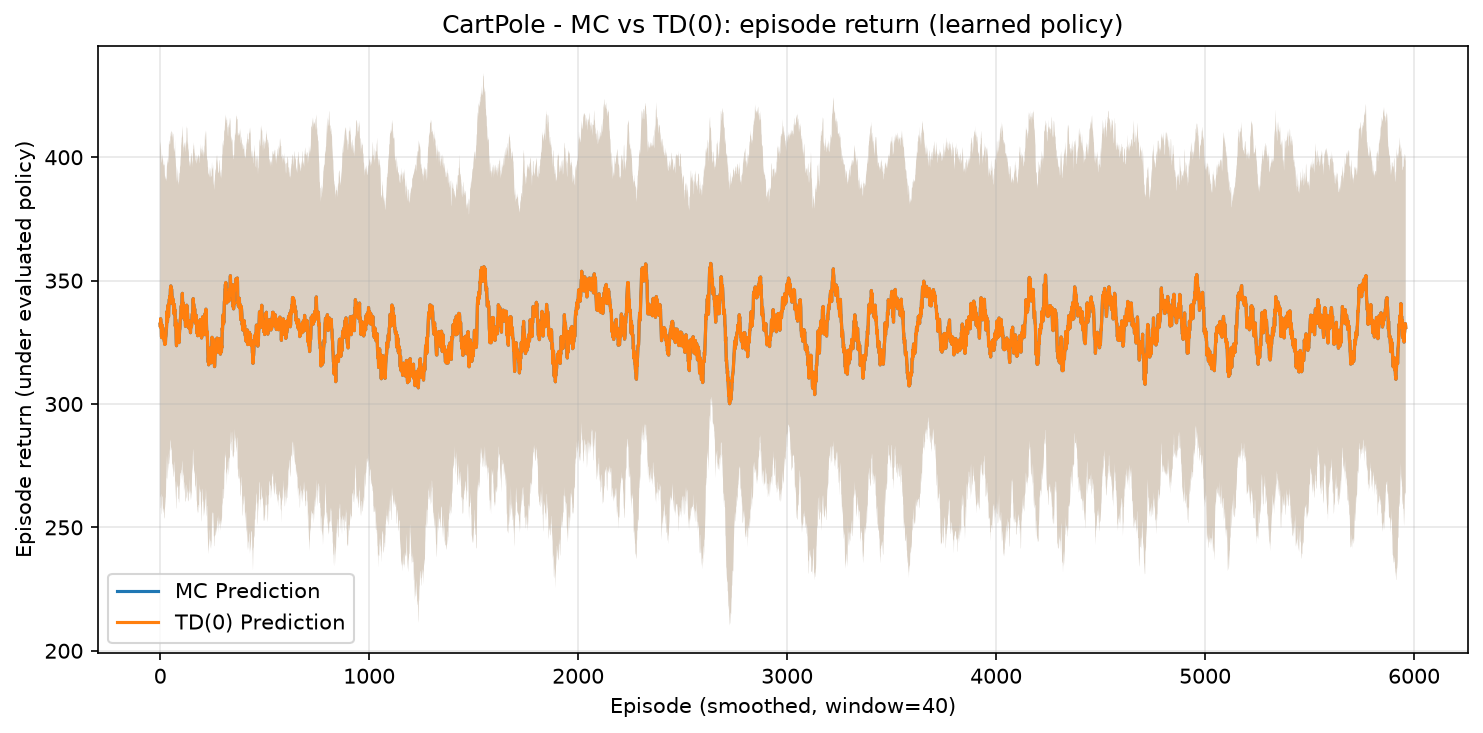
\includegraphics[width=\linewidth]{cartpole_prediction_learned_return.png}
  \caption{Return: identico per costruzione.}
\end{subfigure}\hfill
\begin{subfigure}{0.46\linewidth}
  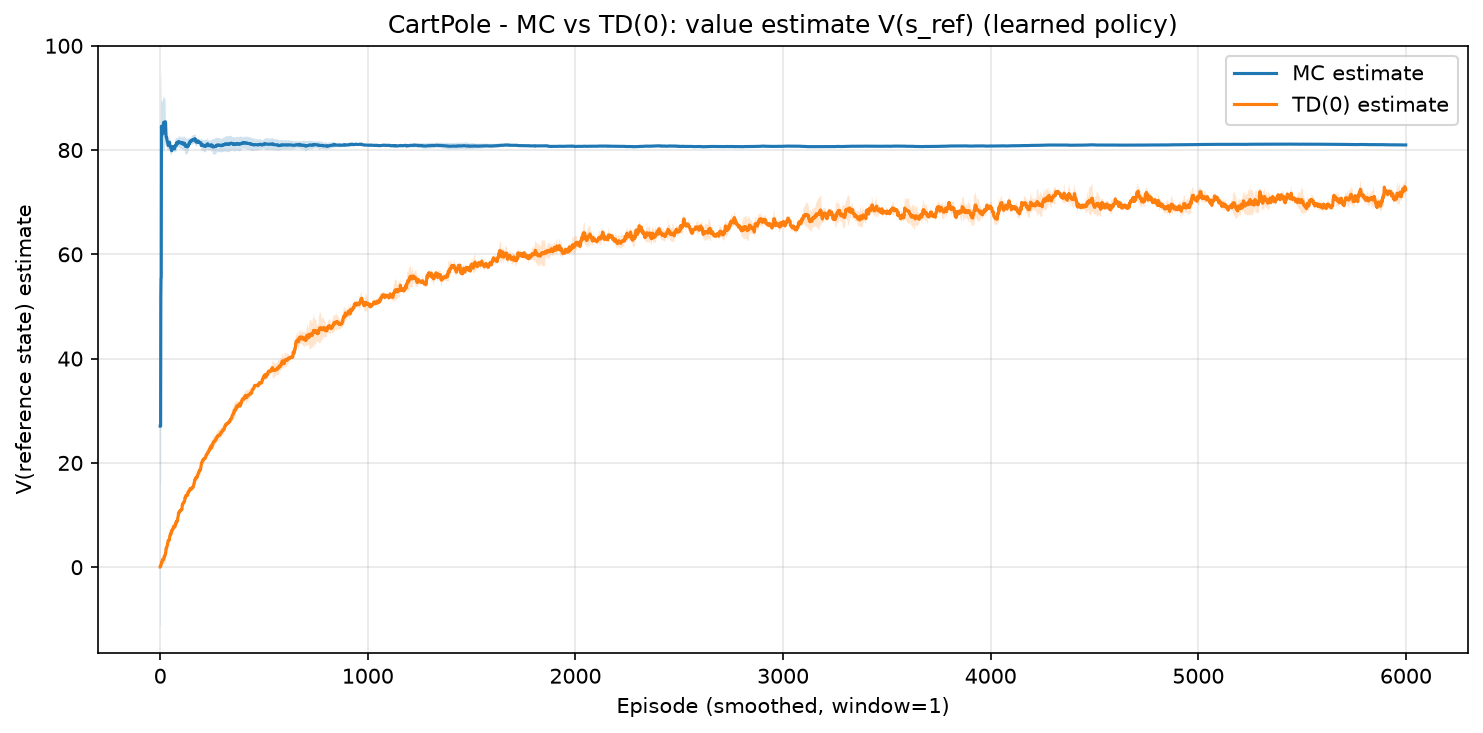
\includegraphics[width=\linewidth]{cartpole_prediction_learned_value.png}
  \caption{Stima $V(s_{\text{ref}})$: qui divergono.}
\end{subfigure}
\caption{CartPole, MC vs TD(0) sulla \textbf{policy appresa}. (a) Stessa policy, stessi
episodi: il return non pu\`o dire nulla sugli stimatori. (b) Le stime invece raccontano
tutto: MC (blu) non distorto e ad alta varianza iniziale, TD(0) (arancio) liscio ma
distorto verso l'inizializzazione e non ancora convergente a 6000 episodi.}
\label{fig:cp-pred}
\end{figure}

\begin{figure}[htbp]
\centering
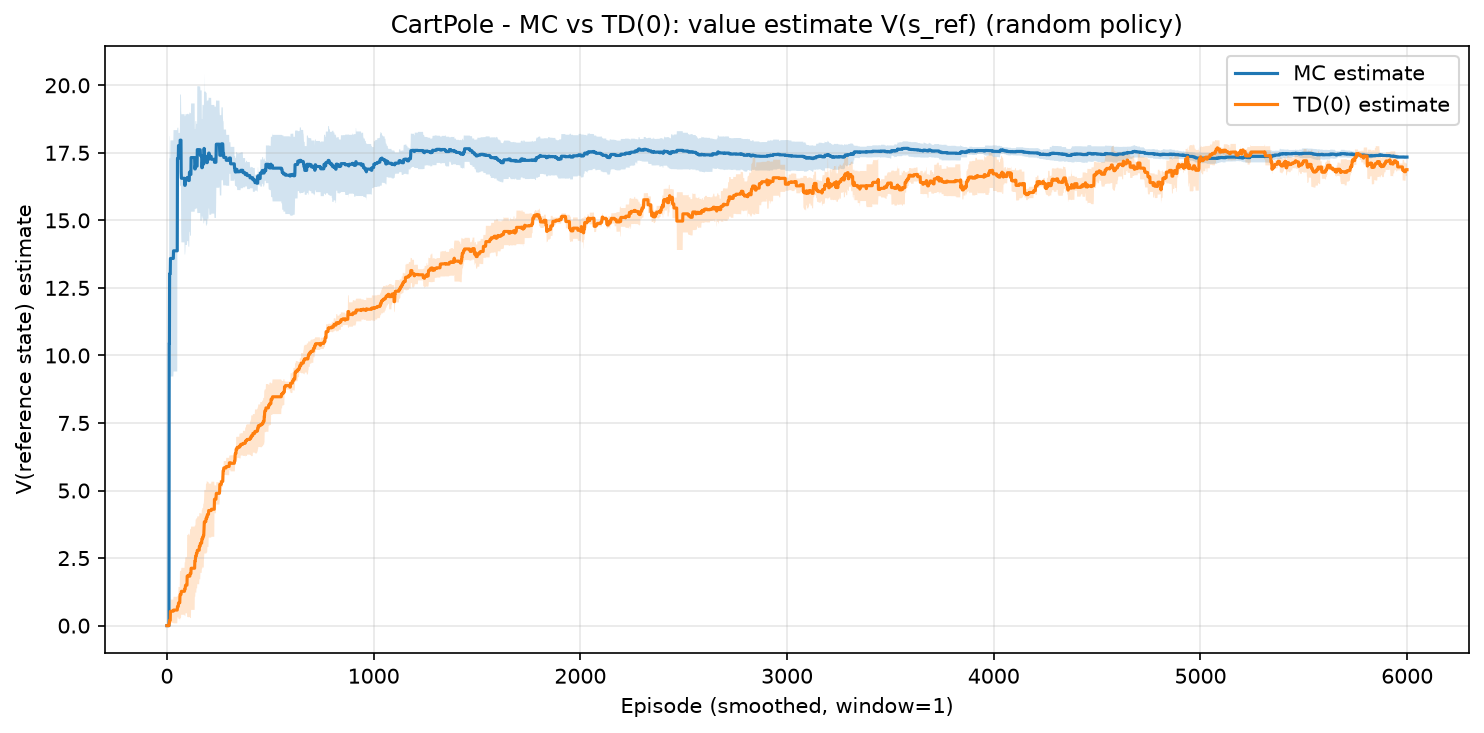
\includegraphics[width=0.52\linewidth]{cartpole_prediction_random_value.png}
\caption{CartPole, MC vs TD(0) sulla \textbf{policy casuale}. Con episodi corti
($\approx 22$ passi) il bootstrap propaga in fretta e TD \emph{raggiunge} MC: il bias
dipende da quanto lo stato \`e lontano dalla terminazione. Da confrontare con la
Fig.~\ref{fig:cp-pred}b.}
\label{fig:cp-pred-random}
\end{figure}

Le figure del return sulla policy casuale e su Acrobot esistono in \code{figures/} ma
non sono riportate: mostrano lo stesso fenomeno di Fig.~\ref{fig:cp-pred}a (curve
sovrapposte per costruzione) e non aggiungono informazione.

% =====================================================================
\subsection{Acrobot --- controllo}
\label{sec:res-acrobot-control}

Entrambi gli algoritmi migliorano da $\approx -470$ (vicino al casuale, $-500$) fino a
\res{-341.4}{27.8} (Q\hbox{-}Learning) e \res{-348.6}{3.2} (SARSA), restando lontanissimi
dall'ottimo ($\approx -100$): l'agente impara qualche spinta utile, non uno swing-up
efficiente (Fig.~\ref{fig:ac-control}, Tab.~\ref{tab:acrobot-control}).

Il dato pi\`u istruttivo \`e la \textbf{forma} della curva: il grosso del miglioramento
avviene entro i primi $\approx 5000$ episodi, poi le curve oscillano attorno a
$-340/-350$ \emph{senza migliorare} per altri 15\,000. Non \`e lentezza, \`e un tetto:
raddoppiare il budget non lo sposta. Con 46\,656 stati e un reward informativo solo
quando l'obiettivo viene raggiunto per caso, la Q-table a 6 bin non ha la risoluzione per
rappresentare una politica migliore --- ipotesi che la sezione seguente verifica.

Notevole l'inversione rispetto a CartPole sulla varianza: qui \`e \textbf{SARSA} ad
essere drasticamente pi\`u stabile ($\pm 3.2$ contro $\pm 27.8$). La stabilit\`a relativa
dei due algoritmi non \`e una loro propriet\`a intrinseca ma dipende dall'ambiente; la
Sez.~\ref{sec:discussion} riprende il punto.

\begin{figure}[htbp]
\centering
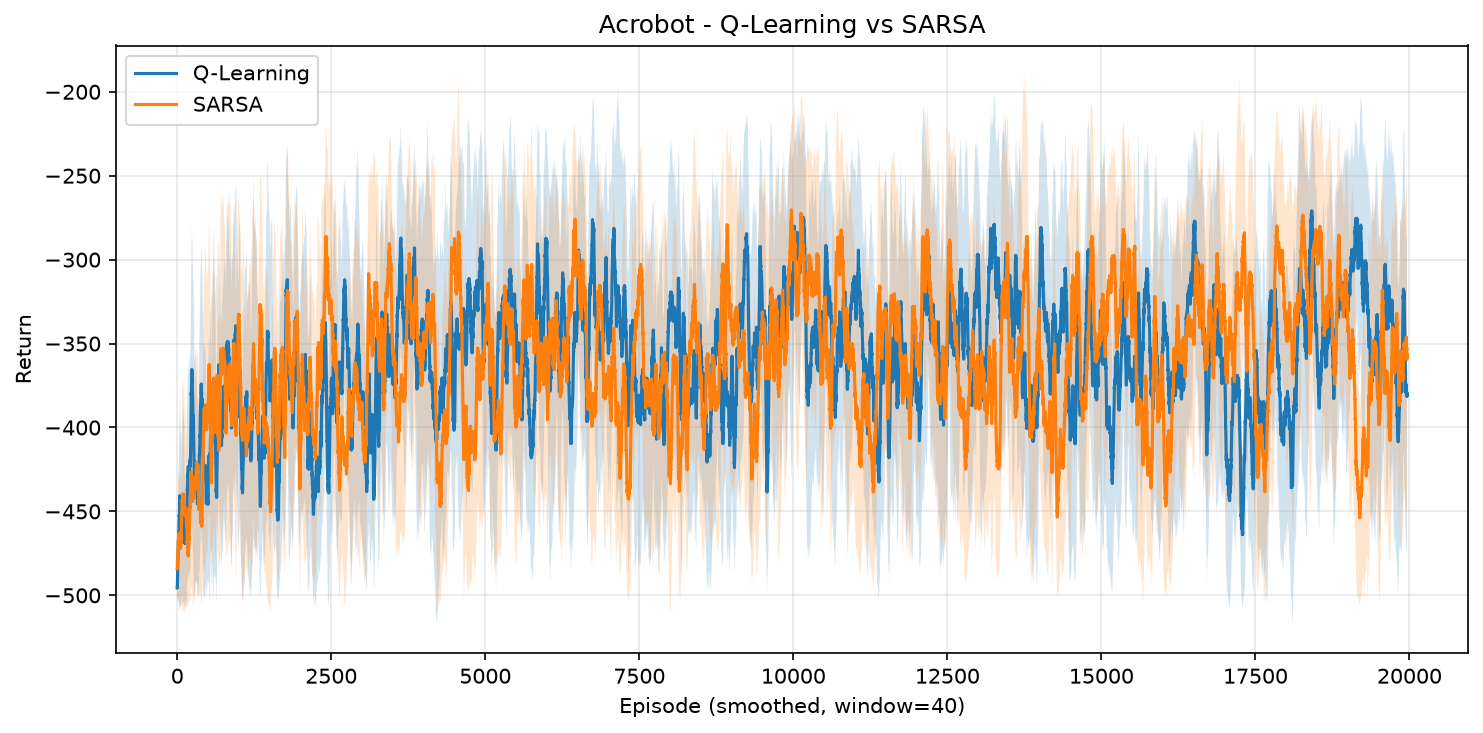
\includegraphics[width=0.55\linewidth]{acrobot_control_comparison.png}
\caption{Acrobot: Q\hbox{-}Learning vs SARSA. Miglioramento reale rispetto al casuale
($-500$), ma plateau precoce ($\approx 5000$ episodi) e molto lontano dall'ottimo
($\approx -100$).}
\label{fig:ac-control}
\end{figure}

\begin{table}[htbp]
\centering
\caption{Acrobot, controllo: Q-Learning vs SARSA, media su 3 seed. Policy casuale $\approx -500$; un buon swing-up raggiunge $\approx -100$.}
\label{tab:acrobot-control}
\begin{tabular}{lccc}
\toprule
Algoritmo & Return iniziale & Return finale & Episodi/seed \\
          & (primi 100 ep) & (ultimo 10\% ep, media $\pm$ std) & \\
\midrule
Q-Learning & -468.0 & $-341.4 \pm 27.8$ & 20000 \\
SARSA & -473.2 & $-348.6 \pm 3.2$ & 20000 \\
\bottomrule
\end{tabular}
\end{table}


% =====================================================================
\subsection{Acrobot --- risoluzione della discretizzazione}
\label{sec:res-acrobot-bins}

\textbf{\`E l'esperimento che ha smentito la mia ipotesi di partenza}, ed \`e il
risultato pi\`u istruttivo del progetto. L'ipotesi: aumentare i bin \emph{peggiora}
l'apprendimento, perch\'e lo spazio cresce come $\text{bin}^6$ e a 10 bin ($10^6$ stati)
la tabella diventa irrimediabilmente sparsa --- la curse of dimensionality da manuale.

I dati dicono l'\textbf{opposto}, in modo monotono e non ambiguo
(Fig.~\ref{fig:ac-bins}): a 20\,000 episodi \textbf{10 bin \`e la configurazione
migliore} ($\approx -280$) e \textbf{4 bin la peggiore} ($\approx -430$), con 8 e 6
ordinatamente in mezzo.

Avevo confrontato il costo sbagliato. Le dinamiche di Acrobot richiedono
\emph{precisione angolare}: con 4 bin per dimensione, configurazioni del pendolo che
richiedono coppie \emph{opposte} finiscono nello \emph{stesso} stato discreto. La
Q-table non pu\`o rappresentare politiche diverse per stati che non sa distinguere, e
nessun numero di episodi lo ripara --- infatti la curva a 4 bin resta piatta e rumorosa
fino in fondo. Questo costo di \emph{aliasing} domina quello della sparsit\`a: la curse
of dimensionality \`e reale in principio, ma a questo budget non \`e ancora il vincolo
attivo. \`E anche la giustificazione empirica del passaggio al DQN: per avere insieme
precisione e generalizzazione serve un approssimatore di funzione.

\begin{figure}[htbp]
\centering
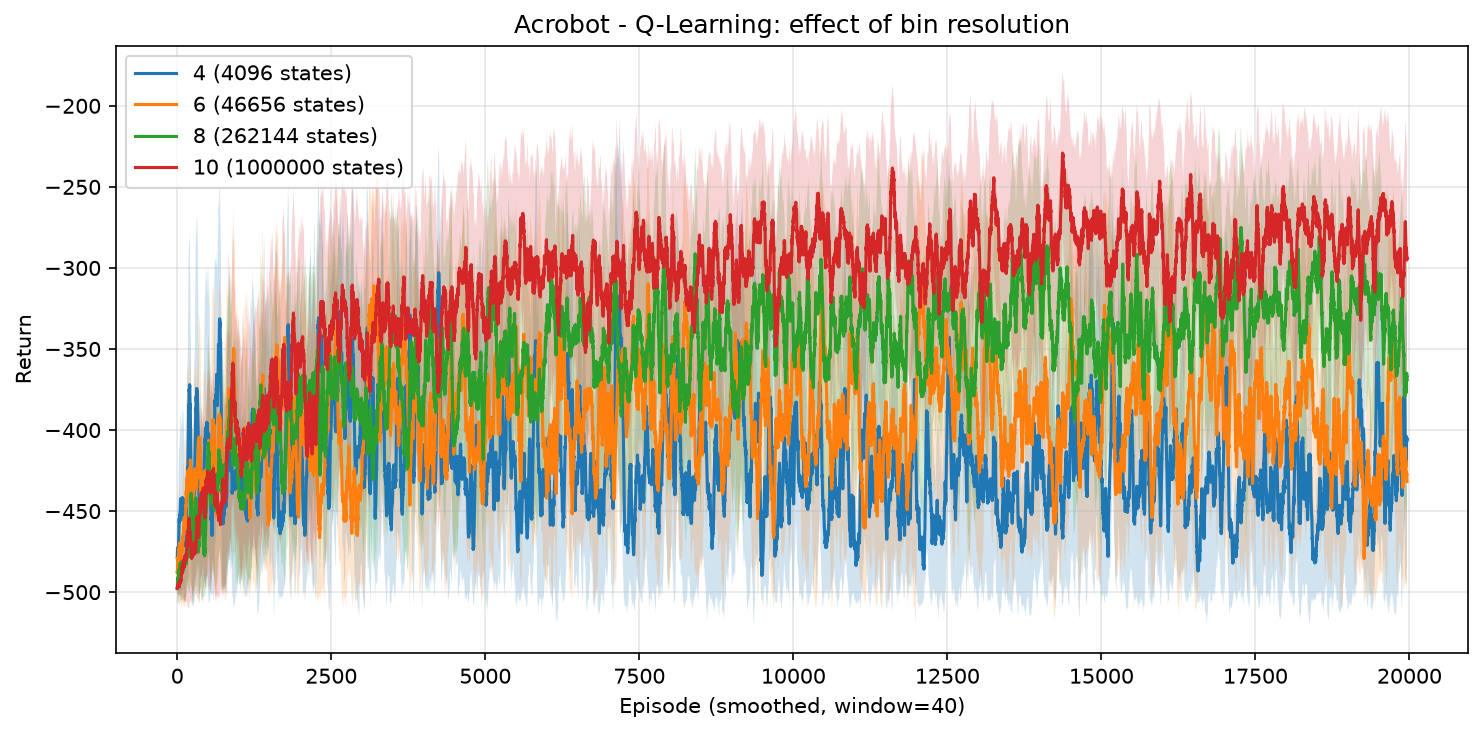
\includegraphics[width=0.55\linewidth]{acrobot_bin_resolution.png}
\caption{Acrobot: effetto della risoluzione di discretizzazione (Q\hbox{-}Learning,
20\,000 episodi). Contrariamente all'ipotesi, 10 bin ($10^6$ stati, rosso) \`e la
configurazione \emph{migliore} e 4 bin (blu) la peggiore, con ordinamento monotono: 4
bin non riescono a distinguere stati che richiedono coppie opposte.}
\label{fig:ac-bins}
\end{figure}

% =====================================================================
\subsection{Acrobot --- esplorazione: $\varepsilon$ costante e annealing}
\label{sec:res-acrobot-eps}

Anche qui l'attesa era chiara --- reward sparso $\Rightarrow$ serve \emph{pi\`u}
esplorazione --- e anche qui la sweep a $\varepsilon$ costante dice il contrario
(Fig.~\ref{fig:ac-explore}a): i valori \emph{bassi} vincono ($\varepsilon = 0.05$ arriva
a $\approx -310$) e $\varepsilon = 0.4$ \`e nettamente il peggiore ($\approx -450$), di
nuovo in ordine monotono.

Il punto non \`e che l'esplorazione sia inutile, ma che \textbf{l'esplorazione
\emph{costante} \`e lo strumento sbagliato}: con $\varepsilon = 0.4$ l'agente continua a
iniettare coppie casuali \emph{anche dopo} aver trovato uno swing-up, distruggendolo ad
ogni episodio.

L'annealing conferma la lettura e chiude il cerchio (Fig.~\ref{fig:ac-explore}b): lo
schedule $1.0 \to 0.01$ raggiunge \res{-316.3}{24.5} contro \res{-341.4}{27.8} del
miglior $\varepsilon$ costante --- il guadagno pi\`u grande ottenuto su Acrobot senza
toccare l'algoritmo. Il prezzo \`e visibile: per $\approx 5000$ episodi la curva annealed
\`e inchiodata a $-500$ (con $\varepsilon \approx 1$ l'agente \`e di fatto casuale),
sorpassa attorno a $9000$ e da l\`i resta sopra. Il confronto con CartPole, dove lo stesso
schedule d\`a un guadagno modesto, isola il meccanismo: l'annealing paga dove
l'esplorazione \`e davvero il collo di bottiglia.

\begin{figure}[htbp]
\centering
\begin{subfigure}{0.46\linewidth}
  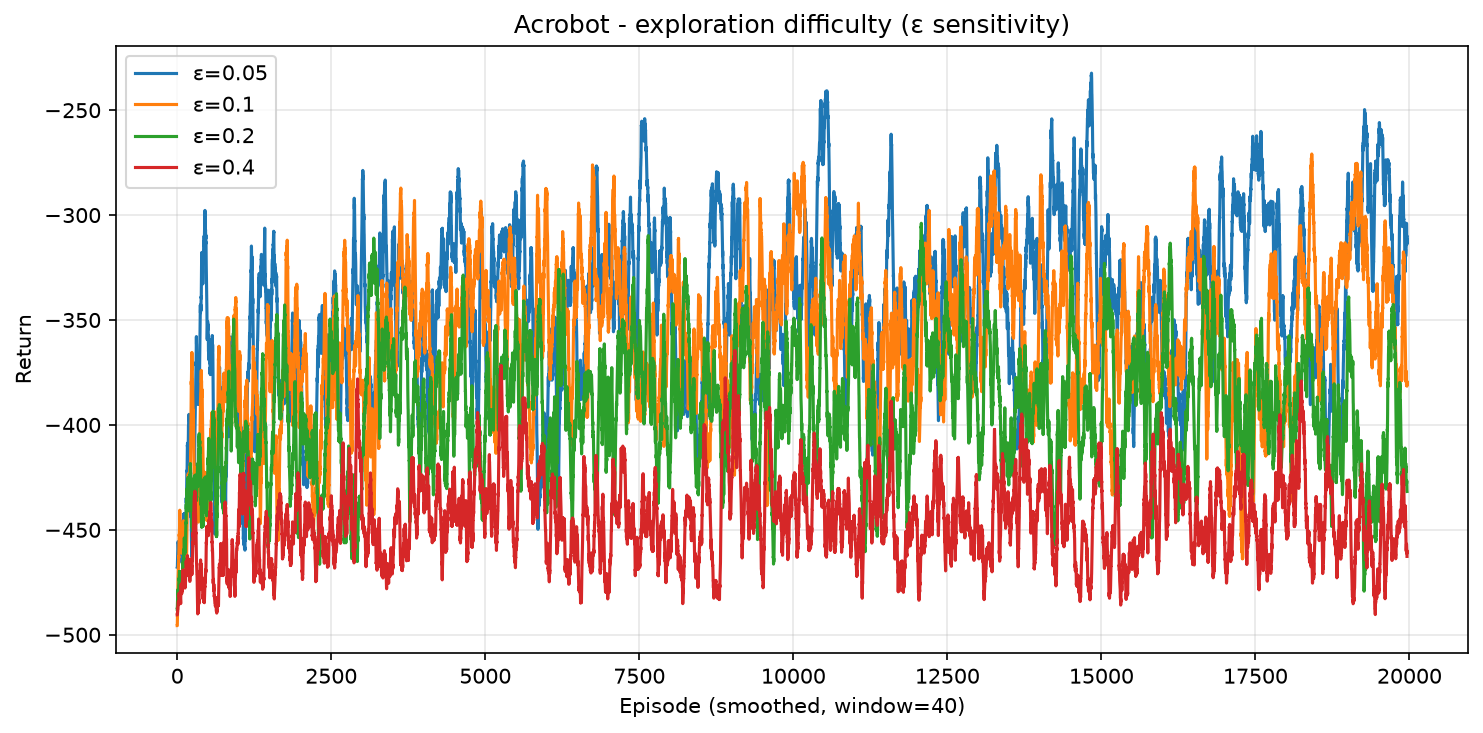
\includegraphics[width=\linewidth]{acrobot_sensitivity_epsilon.png}
  \caption{$\varepsilon$ costante: basso batte alto.}
\end{subfigure}\hfill
\begin{subfigure}{0.46\linewidth}
  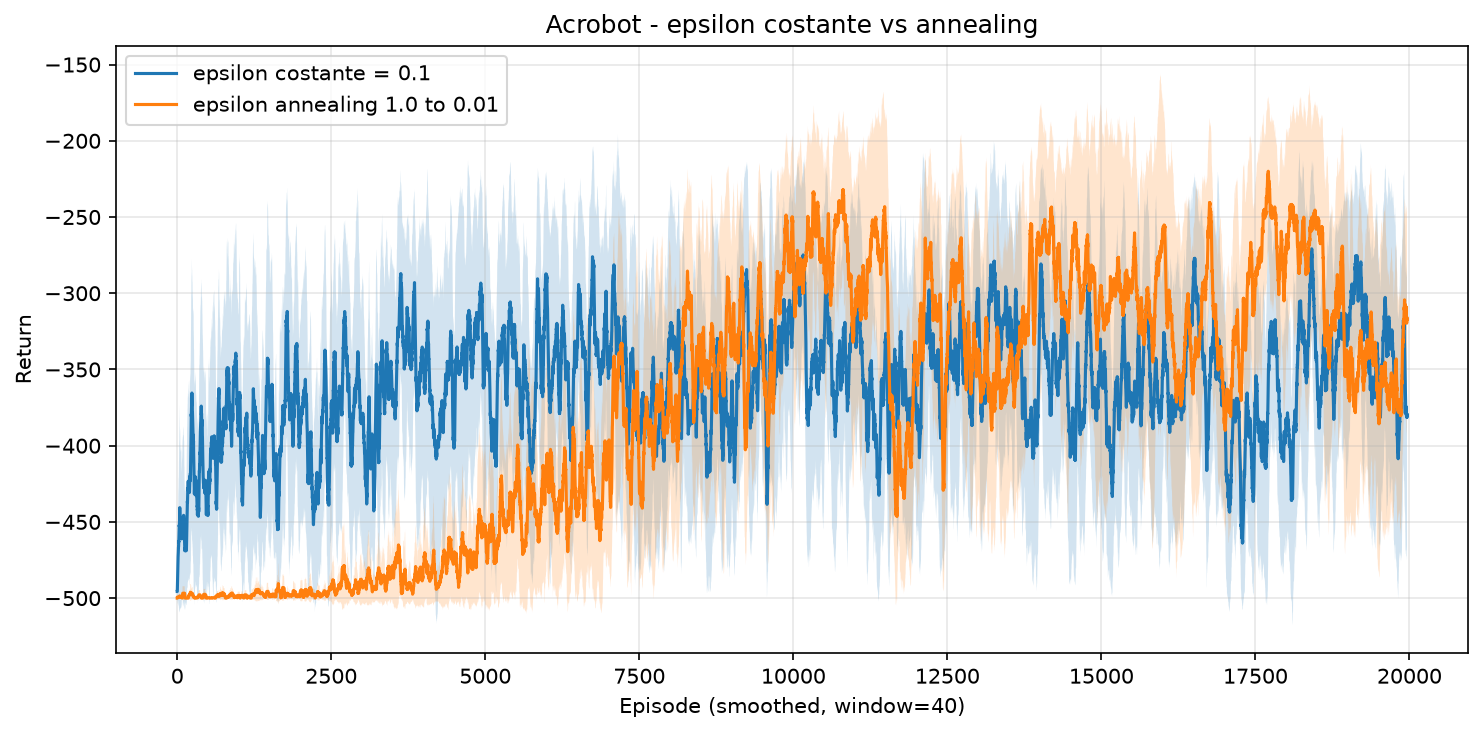
\includegraphics[width=\linewidth]{acrobot_epsilon_annealing.png}
  \caption{Annealing $1.0 \to 0.01$ vs costante $0.1$.}
\end{subfigure}
\caption{Acrobot, esplorazione. (a) A $\varepsilon$ \emph{costante} i valori bassi
vincono: un $\varepsilon$ alto tenuto fisso continua a distruggere lo swing-up appreso.
(b) Ma l'esplorazione \emph{decrescente} \`e la scelta giusta: paga $\approx 5000$
episodi a $-500$ e poi supera stabilmente il miglior $\varepsilon$ costante. Insieme, i
due pannelli dicono che il problema non era ``quanta'' esplorazione, ma ``quando''.}
\label{fig:ac-explore}
\end{figure}

% =====================================================================
\subsection{Acrobot --- MC vs TD(0)}
\label{sec:res-acrobot-pred}

Il bias di TD(0) \`e qui ancora pi\`u marcato che su CartPole (Fig.~\ref{fig:ac-pred}),
e conferma l'interpretazione data sopra. MC converge quasi subito a $-91.17 \pm 0.27$;
TD(0) parte da 0, \emph{scende lentamente} e dopo 6000 episodi \`e solo a
$-62.00 \pm 0.03$. Lo stato di riferimento \`e a $\approx 90$ passi dall'obiettivo e TD
propaga il valore un passo per volta: per uno stato cos\`i distante dal reward il
bootstrap \`e lentissimo e la stima resta ancorata all'inizializzazione.

Si noti la banda: quella di TD(0) \`e cos\`i stretta da risultare invisibile
($\pm 0.03$), quella di MC \`e ampia nei primi episodi. \`E il compromesso bias/varianza
nella sua forma pi\`u pura: TD \`e molto \emph{preciso} nel dare la risposta
\emph{sbagliata}, e ci mette molto ad arrivare a quella giusta.

\begin{figure}[htbp]
\centering
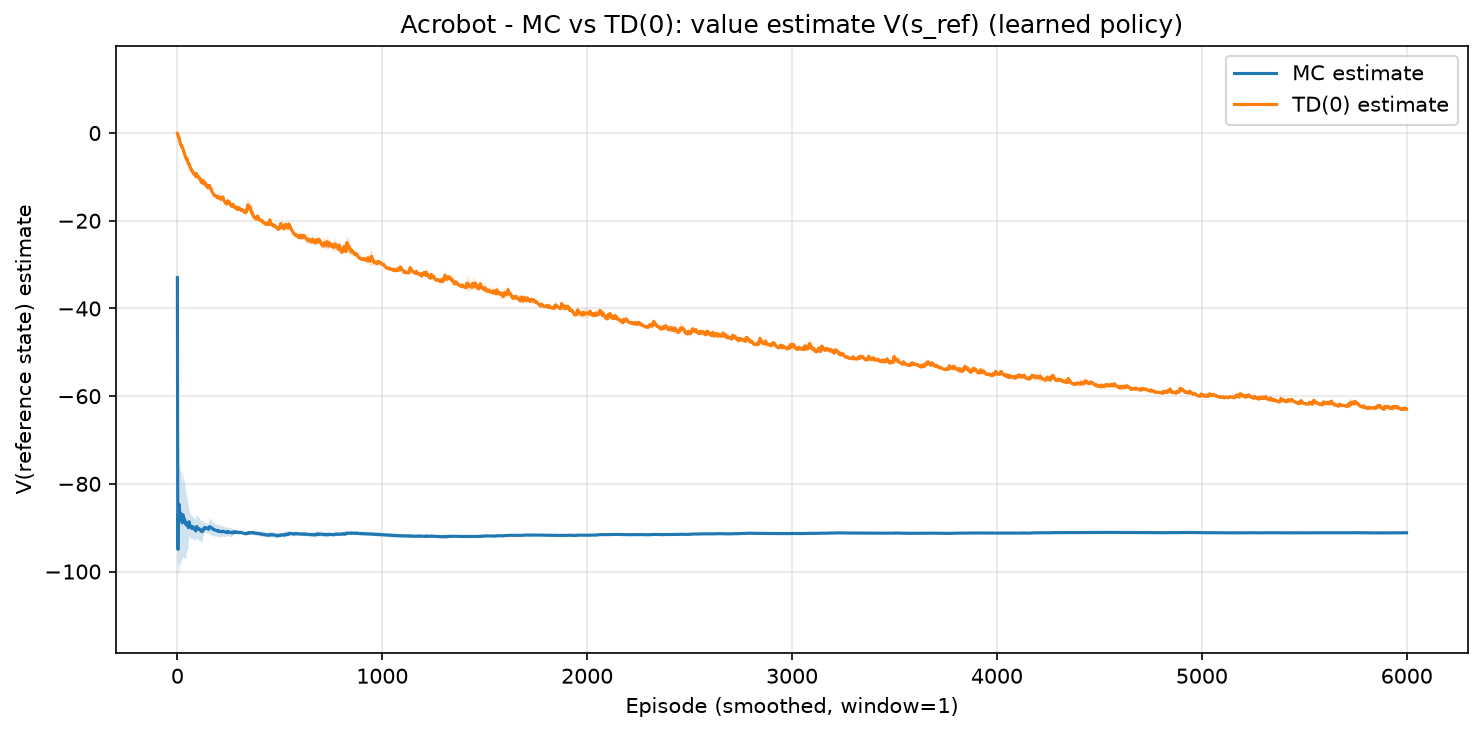
\includegraphics[width=0.54\linewidth]{acrobot_prediction_value.png}
\caption{Acrobot, MC vs TD(0): stima $V(s_{\text{ref}})$ della policy appresa. MC (blu)
converge subito a $\approx -91$; TD(0) (arancio) scende da 0 con estrema regolarit\`a ma
dopo 6000 episodi \`e ancora a $\approx -62$.}
\label{fig:ac-pred}
\end{figure}

% =====================================================================
\subsection{Pong --- ablazione del DQN}
\label{sec:res-pong}

Rispetto alla baseline casuale ($\approx -20.4$) e con soli 200k step
(Fig.~\ref{fig:pong-full}, Tab.~\ref{tab:pong-ablation}):
\begin{itemize}
  \item \textbf{DQN completo}: \res{-12.1}{0.9}. Apprende nettamente e in modo
        consistente tra i seed: il requisito della consegna (``mostrare apprendimento
        rispetto a policy casuale'') \`e soddisfatto con ampio margine.
  \item \textbf{Double DQN} (bonus): \res{-14.2}{0.8}. Apprende, con traiettoria simile
        al completo, senza superarlo.
  \item \textbf{Senza target network}: \res{-16.3}{2.8}. Apprende, ma pi\`u tardi e con
        varianza \emph{tripla}.
  \item \textbf{Senza replay} / \textbf{senza entrambi}: \res{-20.6}{0.2} e
        \res{-20.5}{0.3} --- \emph{nessun apprendimento}, restano al livello casuale.
\end{itemize}

\textbf{I due componenti non sono equivalenti} (Fig.~\ref{fig:pong-ablation}). Il
\emph{replay \`e indispensabile}: senza, la rete si addestra sul flusso di transizioni
consecutive fortemente correlate e in 200k step non impara nulla --- la curva \`e piatta.
La \emph{target network} \`e invece un \emph{acceleratore e stabilizzatore}: senza,
l'agente impara comunque (da $-20.4$ a $-16.3$), ma pi\`u tardi e con varianza tra seed
molto maggiore, il sintomo atteso del ``bersaglio mobile'' (ogni passo di gradiente
sposta anche il target). La distinzione tra componente \emph{necessario} e componente
\emph{utile} \`e il contenuto informativo dell'ablazione.

Un segnale indiretto ma elegante: il DQN completo produce \emph{meno} episodi per seed
($134$) delle configurazioni fallite ($\approx 240$). A parit\`a di step, un agente che
impara tiene in vita gli scambi pi\`u a lungo e gioca quindi meno partite: il numero di
episodi \`e esso stesso una misura di apprendimento.

Sul \textbf{Double DQN}: non supera il DQN base, ed \`e un esito spiegabile. Corregge la
\emph{sovrastima} dovuta al $\max$ su stime rumorose, un problema che si accumula su
orizzonti lunghi; a 200k step (lo $0.4\%$ del budget Nature) non ha ancora avuto tempo
di fare danno. Il bonus \`e implementato e funzionante --- semplicemente, in questo
regime, non c'\`e il male che dovrebbe curare.

\begin{figure}[htbp]
\centering
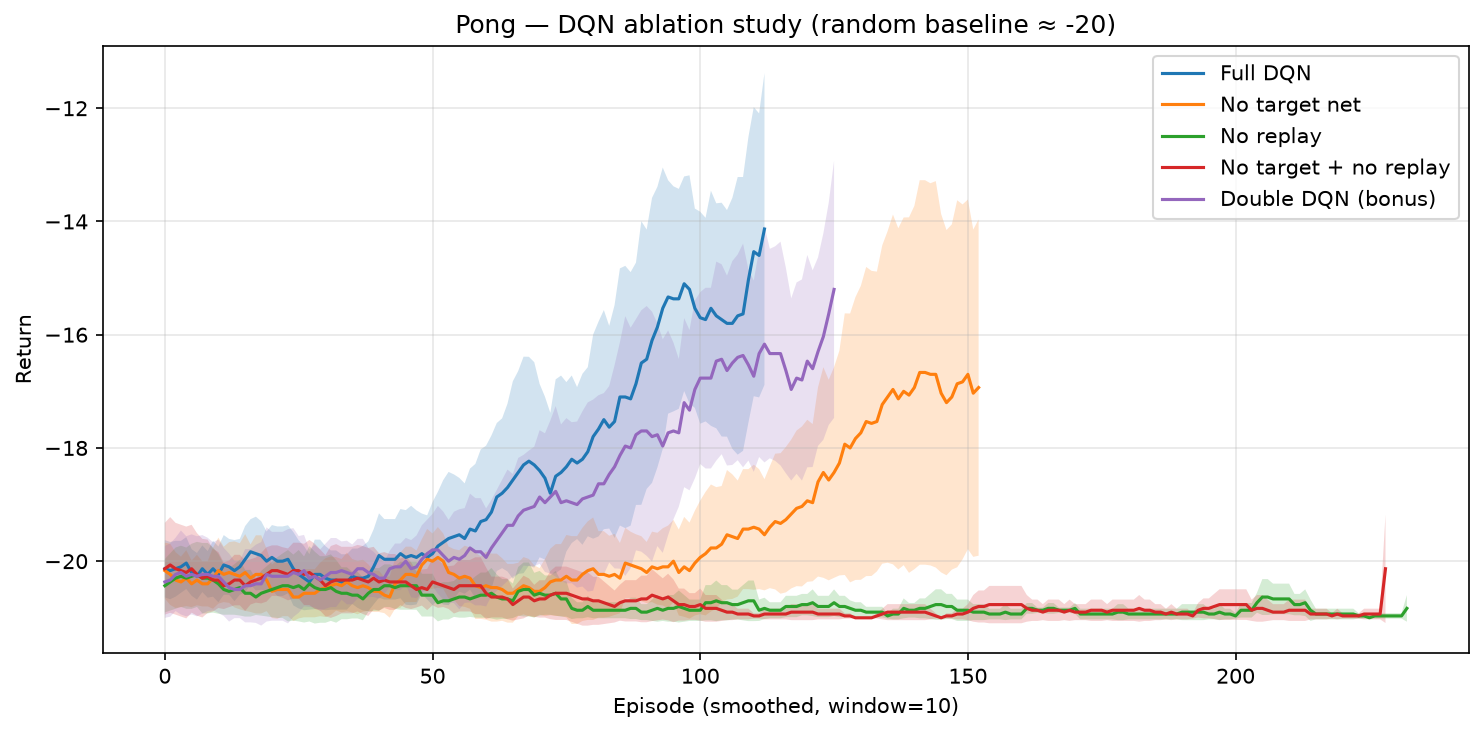
\includegraphics[width=0.55\linewidth]{pong_full_comparison.png}
\caption{Pong: ablazione DQN completa (200k step, 3 seed, baseline casuale
$\approx -20$). DQN completo (blu) e Double DQN (viola) apprendono; senza target network
(arancio) si impara pi\`u tardi e peggio; le due configurazioni senza replay (verde e
rosso) restano piatte al livello casuale.}
\label{fig:pong-full}
\end{figure}

\begin{figure}[htbp]
\centering
\begin{subfigure}{0.46\linewidth}
  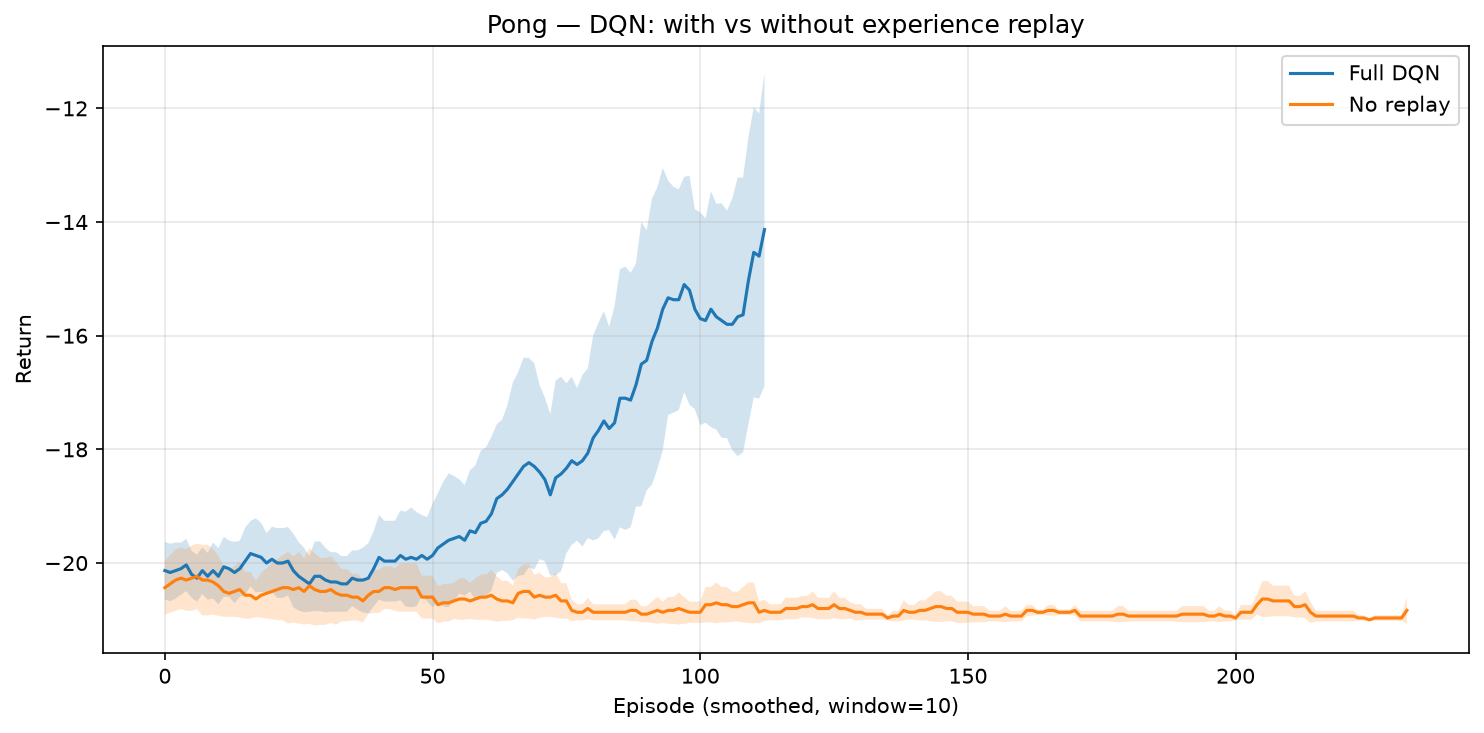
\includegraphics[width=\linewidth]{pong_ablation_replay.png}
  \caption{Con vs senza experience replay.}
\end{subfigure}\hfill
\begin{subfigure}{0.46\linewidth}
  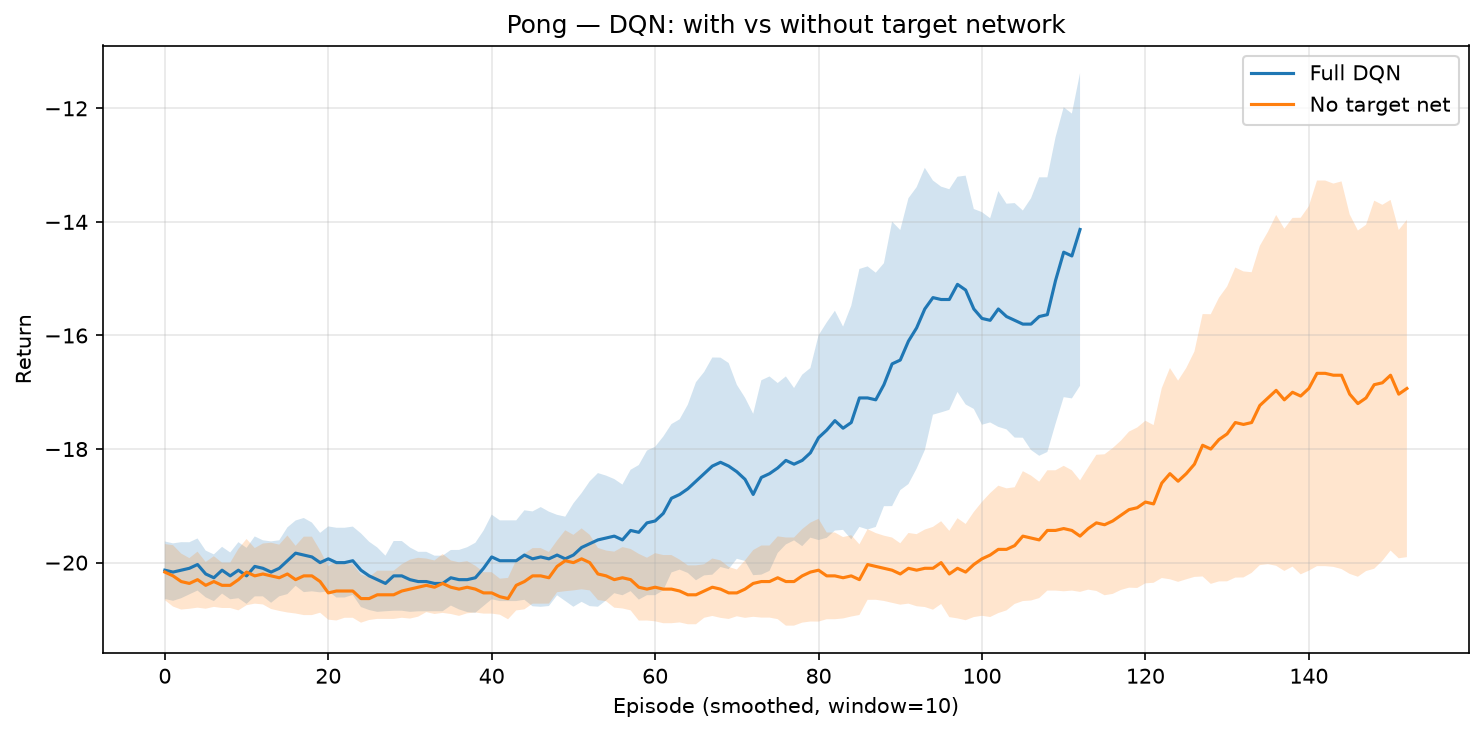
\includegraphics[width=\linewidth]{pong_ablation_target.png}
  \caption{Con vs senza target network.}
\end{subfigure}
\caption{Pong: le due ablazioni richieste dalla consegna, isolate. (a) Senza replay la
curva non si stacca mai dal livello casuale: componente \emph{necessario}. (b) Senza
target network l'apprendimento avviene, ma pi\`u tardi e con banda $\pm1\sigma$ molto
pi\`u larga: componente \emph{stabilizzante}.}
\label{fig:pong-ablation}
\end{figure}

\begin{table}[htbp]
\centering
\caption{Ablazione DQN su Pong: performance finale dopo 200k step ambiente, media $\pm$ std su 3 seed. Policy casuale $\approx -20.4$.}
\label{tab:pong-ablation}
\begin{tabular}{lcc}
\toprule
Configurazione & Return finale & Episodi/seed \\
               & (ultimo 10\% ep, media $\pm$ std) & (media) \\
\midrule
DQN completo (replay + target) & $-12.1 \pm 0.9$ & 134 \\
Double DQN (bonus) & $-14.2 \pm 0.8$ & 154 \\
Senza target network & $-16.3 \pm 2.8$ & 187 \\
Senza experience replay & $-20.6 \pm 0.2$ & 243 \\
Senza target + senza replay & $-20.5 \pm 0.3$ & 238 \\
\bottomrule
\end{tabular}
\end{table}

